\chapter{Cargas de trabajo}\label{int}
\thispagestyle{fancy}


\section{Resumen de cargas de trabajo}
A continuación, se presentan y detallan las cargas de trabajo que se derivan de cada una de
las tareas del proyecto.
\begin{enumerate}
    \item Investigación inicial
    \item Creación del bot
    \item Puesta en marcha del bot
    \item Crear web
    \item Crear el modelo para almacenar datos en la web
    \item Implementar API DE Google en la web
    \item Implementar lógica de la web
    \item Investigación sobre técnicas para procesar imágenes
    \item Procesar imagen
    \item Conectar bot con la web
    \item Optimizar y mejorar código del proyecto
    \item Redactar memoria
\end{enumerate}
\section{ Diagrama de Gant}
\begin{figure}[h]
\centering
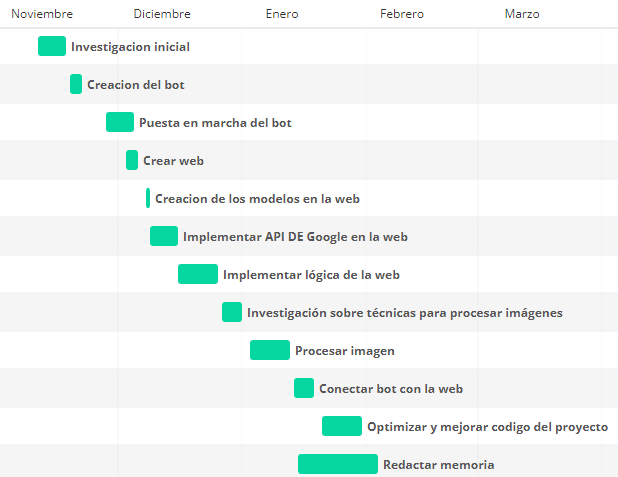
\includegraphics[scale=0.75]{imgs/gant.png}
\end{figure}